% RESULTADOS -------------------------------------------------------------------

\chapter{RESULTADOS}
\label{chap:resultados}

Neste capítulo são apresentados os resultados colhidos neste estudo, organizados pelas questões de pesquisa.

% TIPO DE LICENÇAS ENCONTRADA ------------------------------------------------

\section{Qual o panorama geral do uso de licenças em projetos de software livre JavaScript?}

% MAIS DE UMA LICENÇA --------------------------------------------------------
%\section{Qual a proporção de projetos com mais de uma licença?}
Dentro do universo de analise de projetos, foi criado uma analise com o percentual de projeto com mais de uma licença. 
\gnote{todas as figuras e tabelas precisam ser mencionadas no texto. rever todo o trabalho}

\begin{figure}[H]
    \centering
    \caption{Proporção de projetos com mais de uma licença - Geral}
    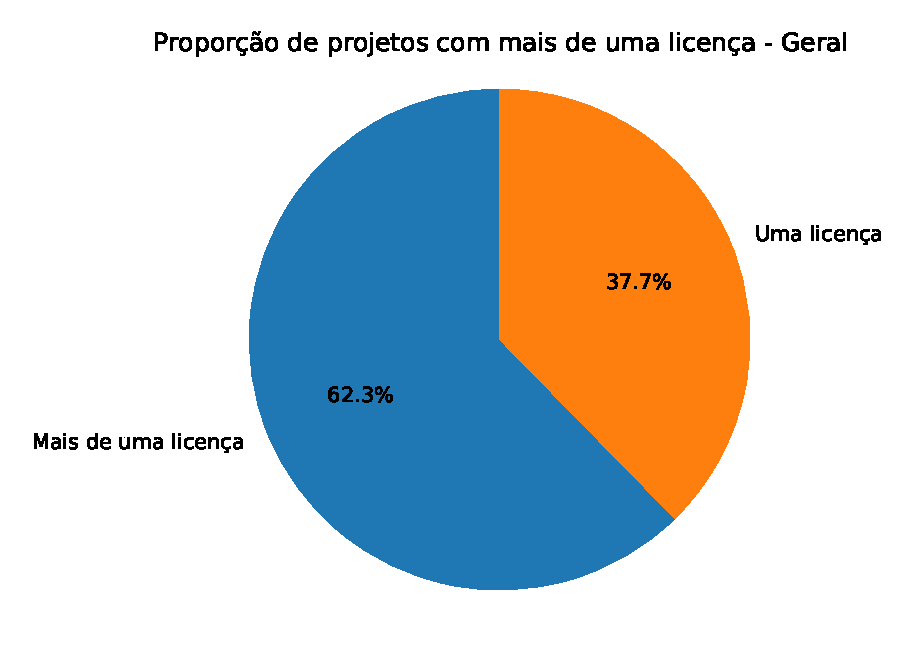
\includegraphics[scale=0.8]{figuras/resultados/pizza_lic_geral.eps}
    \fonte{Autoria própria.}
    \label{local-licencas-raiz}
\end{figure}

A Figura~\ref{local-licencas-raiz} apresenta a proporção de projetos com mais de uma licença. Como pode ser observado, cerca de 38\% dos projetos (582 projetos) apresentam somente uma licença, enquanto que a maioria, mais de 62\% dos projetos (963 projetos), apresenta mais de uma licença. 

%Quando se analisou a quantidade de projetos com mais de uma licença no seu panorama geral, o resultado obtido foi que mais de 60\%  dos analisados apresentaram mais de uma licença contra menos de 40\%.

\begin{figure}[H]
    \centering
    \caption{Proporção de projetos com mais de uma licença - Raiz}
    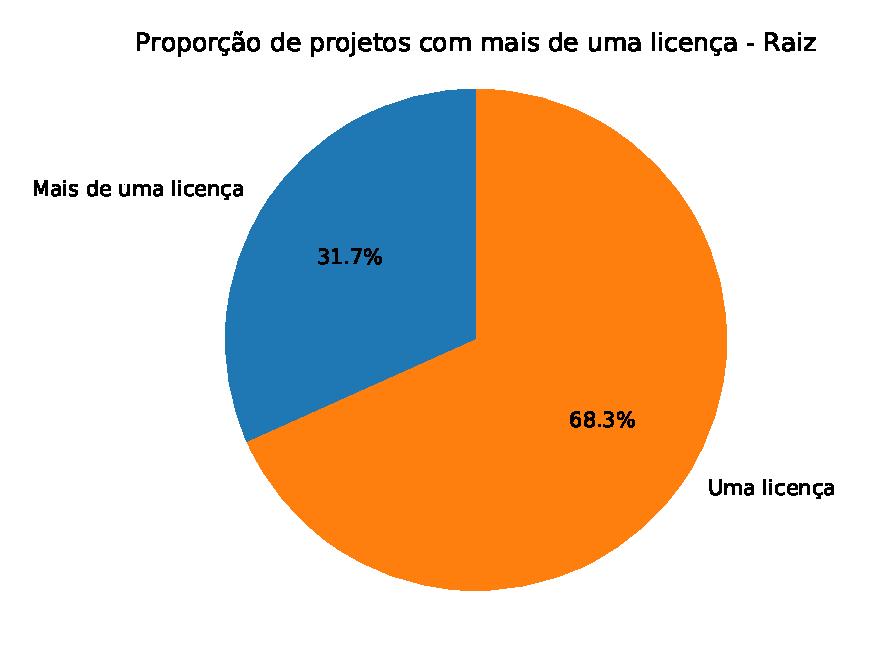
\includegraphics[scale=0.8]{figuras/resultados/pizza_lic_raiz.eps}
    \fonte{Autoria própria.}
    \label{local-licencas-raiz}
\end{figure}

No entanto, é conhecido que desenvolvedores usam diferentes abordagens para declarar licenças de software livre em seus projetos \gnote{citar: http://gustavopinto.org/lost+found/msr2018b.pdf}. Por exemplo \gnote{citar exemplos com detalhes, pe readme, license, outras pastas, etc.}. Dessa forma, foi feito uma nova análise do uso de licenças, mas agora considerando somente as licenças encontradas nas raízes dos projetos. \gnote{mas o label da figura anterior da entender que ela que é na raiz. esse texto é da raiz ou anterior? ajeitar.}
Dessa forma, obtivemos um cenário diferente, onde quase 70\% (1.055 projetos) apresentaram apenas uma licença, ao passo que cerca de 30\% (490 projetos) que apresentam mais de uma licença. Essa análise sugere que desenvolvedores frequentemente não declaram na raiz do projeto todas as licenças utilizadas. Dessa forma, ferramentas que levam em consideração somente licenças declaradas nas raiz potencialmente perdem uma quantidade importante de licenças declaradas em projetos de software livre.

\subsection{Licenças na raiz vs em subdiretórios} \gnote{mover essa subsecao para o local mais adequado}

Para melhor entender o contexto em que licenças são declaradas em subdiretórios dos projetos, foi feita uma análise manual de xxx projetos \gnote{colocar numero}. Após essa análise, foi-se observado três principais principais motivos:

 \begin{itemize}
   \item Muitas das licenças encontradas nos subdiretórios são provenientes de dependências dos projetos. %Com isso licenças de outras projetos.  
   Por exemplo, foi percebido que o projeto tablesaw\footnote{Tablesaw é um projeto do Filament Group que consiste em um conjunto de plugins para criação de tabelas responsivas. Disponível em: \url{https://github.com/filamentgroup/tablesaw/}}, que usa a licença MIT no arquivo LICENSE e no arquivo de package.json, faz uso também da licença Apache\gnote{versao}, no interior de seus diretórios. Isso acontece por causa do uso de bibliotecas externas que foram inseridas no código. Nesse caso em particular, foi adicionado a biblioteca qunit.js, que tem licença MIT e Apache, fazendo com que o projeto tablesaw também adotasse a licença Apache.
   
   \item Licenças provenientes de documentações, como as licenças Creative Commons. Foi percebido que o projeto AngularJs\footnote{AngularJS é um framework JavaScript código aberto, mantido pelo Google, que auxilia na execução de single-page applications. Disponível em: \url{https://github.com/angular/angular}}, usa a licença MIT no arquivo LICENSE e no arquivo de package.json, faz uso também da licença Creative Commons, no interior de seus diretórios. Isso acontece por causa do uso licenças em arquivos de documentação. 
   
   \item Licenças provenientes de exemplos onde o criador especificou uma licença para uso de tal exemplo. Foi percebido que o projeto Gatsby\footnote{Gatsby é um framework gratuito e de código aberto baseado no React que ajuda os desenvolvedores a criar sites e aplicativos rápidos. Disponível em: \url{https://github.com/gatsbyjs/gatsby}}, usa a licença MIT no arquivo LICENSE e no arquivo de package.json, foram encontradas outras licenças MIT no interior de seus diretórios\gnote{nao entendi? ele nao esta usando a mesma licença, mesmo que declarada mais de uma vez? qual o problema?}. Isso acontece por causa do uso licenças em arquivos de exemplo. 
 \end{itemize}

% DISTRIBUIÇÃO DE FREQUENCIA DE LICENÇAS ------------------------------------

\subsection{Quantidade de projetos com mais de uma licença}

Em seguida, foi estudado a proporção de licenças por projeto JavaScript. 
Os resultados da distribuição de frequência estão apresentados na Figura~\ref{local-licencas-raiz}. Nesta figura os outliers foram filtrados para que não ocorra prejuízos na interpretação dos dados. No entanto, os outliers não foram removidos dos dados brutos.

\begin{figure}[H]
    \centering
    \caption{Distribuição de frequência da licenças encontradas em todos os projetos. Outliers foram removidos para que não ocorra prejuízos na interpretação dos dados.}
    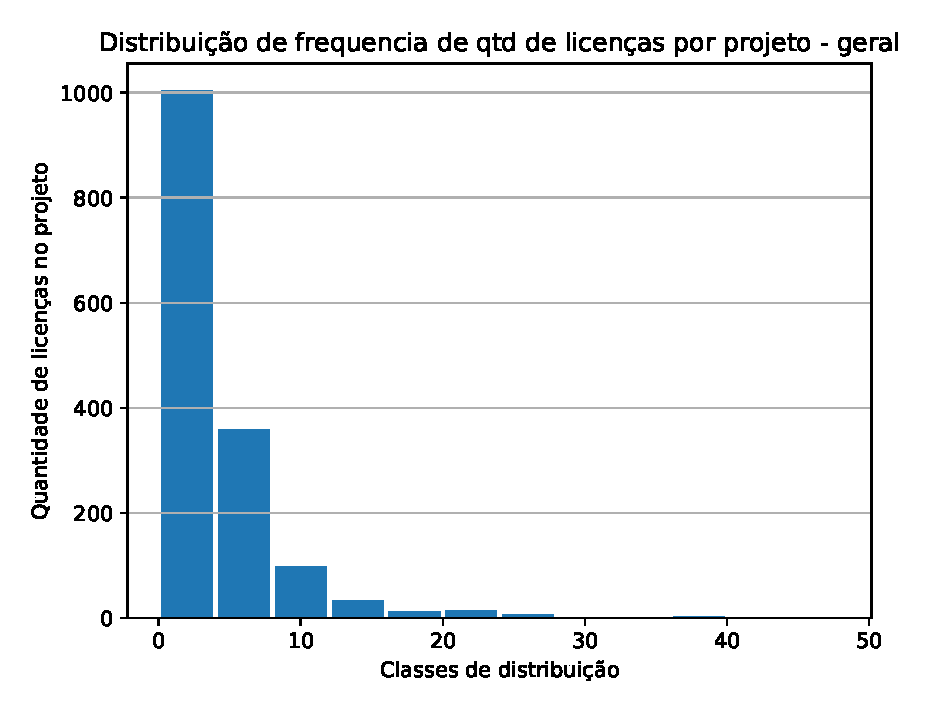
\includegraphics[scale=0.8]{figuras/resultados/hit_qtd_projeto.eps}
    \fonte{Autoria própria.}
    \label{local-licencas-raiz}
\end{figure}


Diante dos resultados observou-se que nas licenças encontradas, no contexto geral de cada projeto analisado, concentra-se entre no intervalo entre 1 e 10 licenças por projeto.\gnote{quantos projetos até 10 licenças?}
No entanto, nesta analise foram encontrados 7 projetos com mais de 50 licenças, entre um intervalo de 86 a 256. Dentre os projetos com mais de 50 licenças, detacam-se xxx (com xxx licenças), xxx (com xxx licenças) e xxx (com xxx licenças).\gnote{complemetnar}

Ademais, estudou-se novamente a distribuição de licenças, considerando somente a declaração de licenças feitas na raiz do projeto. 
Já nessa analise foram encontrados apenas 19 projetos com mais de 7 licenças, reforçando o achado anterior que apresentou que muitas licenças de software livre não são declaradas na raiz do projeto. 
%Compreendendo um intervalo entre 8 e 43 licenças por projeto, com isso esses valores foram removidos como outlier para facilitar a visualização dos dados. 
Nesse contexto, observou-se que existe uma grande concentração de projetos entre o intervalo entre 1 e 2 licenças.\gnote{quantos projetos até 2 licenças?}

\begin{figure}[H]
    \centering
    \caption{Distribuição de frequência da licenças encontradas apenas na raiz dos projetos}
    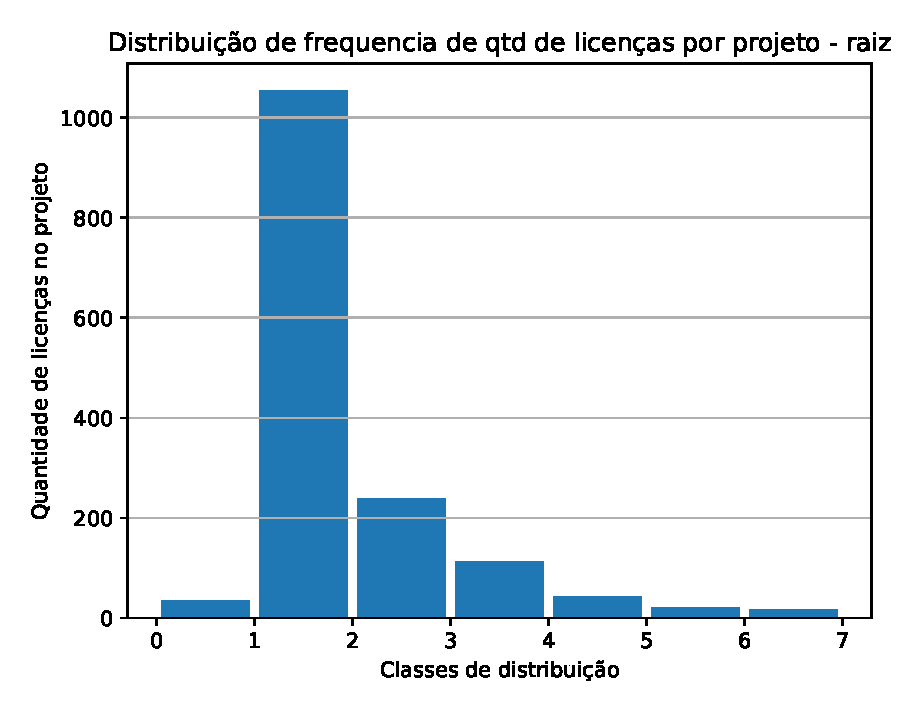
\includegraphics[scale=0.8]{figuras/resultados/hit_qtd_raiz.eps}
	\fonte{Autoria própria.}
    \label{local-licencas-raiz}
\end{figure}


\subsection{Uso de licença não-software} 

%\section{Qual o quantitativo de licenças (de software e não-software) encontradas nos projetos?}

Como foi observado anteriormente, uma parte das licenças encontradas em sub-diretórios não era licença de software (como a Creative Commons). Para melhor entender a existência e uso dessas licenças, foi feito uma uma analise para categorizar as licenças como (1) licenças de software e (2) não-software (licenças de documentação, patente, etc). Para definir as licenças de software, foi utilizado os sites xxx e yyy que fornecem essa descrição, bla bla bla\gnote{complementar}. A Figura~\ref{local-licencas-raiz} apresenta o resultado encotnrado.



\begin{figure}[H]
    \centering
    \caption{quantitativo de licenças (de software e não software) - Geral}
    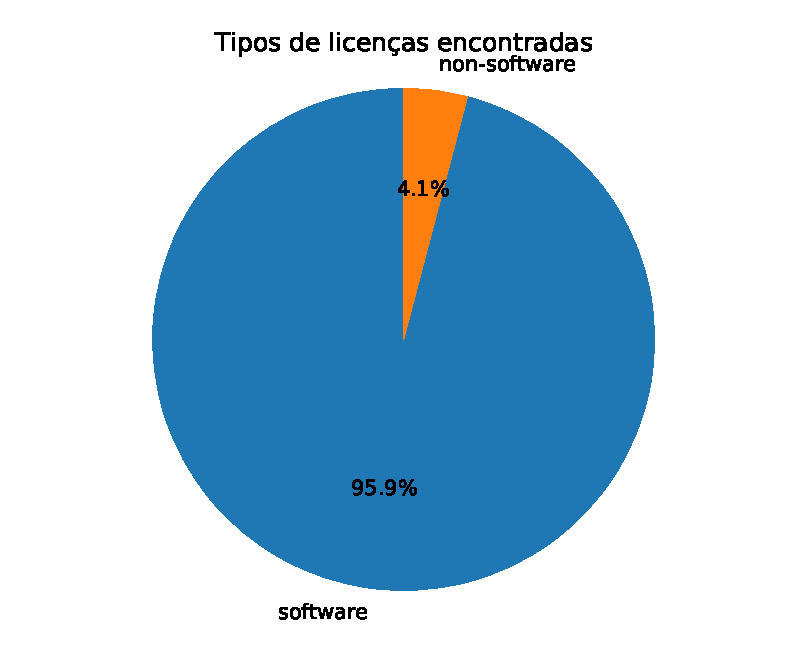
\includegraphics[scale=0.8]{figuras/resultados/tipos_licenca.eps}
    \fonte{Autoria própria.}
    \label{local-licencas-raiz}
\end{figure}

Como se pode observar,  mais de 95\% (248.596 licenças) dos analisados são licenças de software contra apenas de 5\% (10.618 licenças) sendo licenças categorizadas como sendo não-software. Dentre as principais licenças de não-software encontradas, destacam-se as licenas xxx (xxx ocorrencias), xxx (xxx ocorrencias) e xxx (xxx ocorrencias). \gnote{descrever}


% LOCALIZAÇÃO DAS LICENÇAS ---------------------------------------------------
\section{Onde desenvolvedores declaram as licenças?}

Com o intuito de esclarecer os principais arquivos onde foram encontrada as licenças de software livre, foi agrupados os resultados em três arquivos: o license, o readme, e o package.json. O license, como seu nome sugere, é o arquivo principal, no que se refere a declaração de licenças de software livre. Seu uso é extremamente difundido \gnore{citação} e sítios como o GitHub automaticamente inferem estes arquivos para identificar as licenças descritas. O arquivo readme, por outro lado, apresenta uma descrição geral do projeto, geralmente para novos desenvolvedores que querem se ambientar e/ou contribuir com o projeto. Este arquivo também é frequentemente utilizado para declarar as licenças de um projeto, embora não seja necessáriamente obrigatório \gnote{leia a introducao esse arquivo: e melhore o texto como necesario https://ctreude.files.wordpress.com/2018/09/emse18.pdf}. Por fim, o arquivo package.json é a porta de entrada do sistema de gerenciador de pacotes NPM. Além da licença, esse arquivo declara informações como xxx \gnote{complementar}. Se uma licença for declarada, após o deploy do pacote no NPM, os usuários que navegam pelo sítio do NPM poderão identificar o uso dessa licença diretamente no sitio, sem precisarem navegar pelo código fonte ou acessar outros sites (como o GitHub). Em todos os casos, é responsabilidade do mantenedor de projetos adicionar as informações de licença nesses arquivos.
A Figura~\ref{local-licencas-raiz} apresenta a distribuição das licenças entre os arquivos mencionados. Ainda, é apresentado uma barra com ''outros'', o que significa a declaração da licença em outros arquivos.

\begin{figure}[H]
    \centering
    \caption{localização das licenças encontradas na raiz dos projetos}
    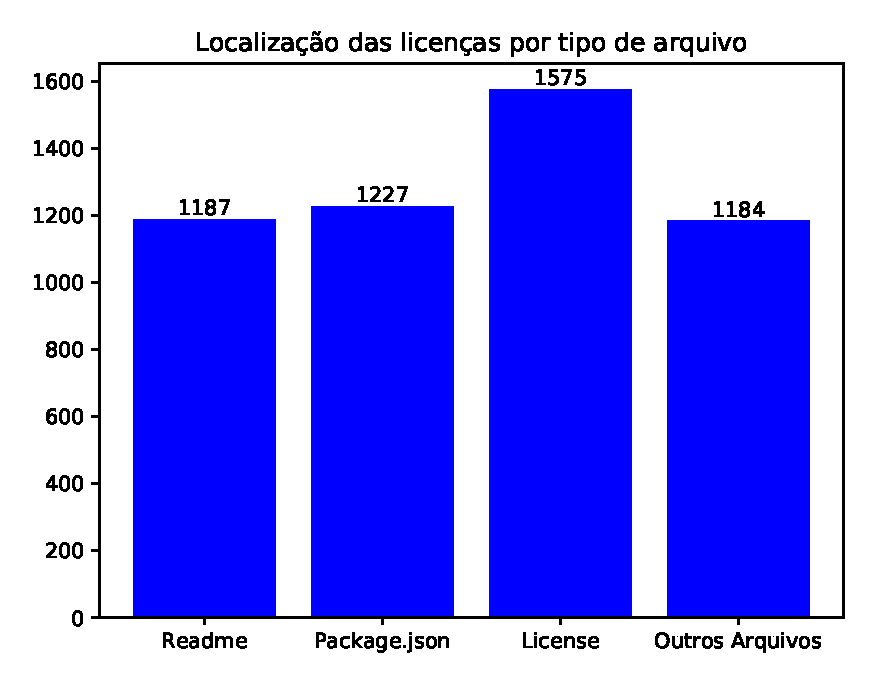
\includegraphics[scale=0.8]{figuras/resultados/barras_local_licencas.eps}
	\fonte{Autoria própria.}
    \label{local-licencas-raiz}
\end{figure}

Como observa-se, a maioria das licenças foram encontradas em arquivos do tipo ``license". Pode se observar também, que essa quantidade é superior a quantidade de projetos analisados, pois existem projetos que apresentam mais de uma licença e cada licença é listada em um arquivo individual. Como um exemplo, detaca-se o projeto Annotator\footnote{Annotator é uma biblioteca JavaScript para criar aplicativos de anotação em navegadores. Ele fornece um conjunto de ferramentas interoperáveis para anotar conteúdo em páginas da web. Link do projeto: \url{https://github.com/openannotation/annotator}}, que apresenta a licença MIT em um arquivo nomeado "LICENSE-MIT" e a licença GLP em um outro arquivo "LICENSE-GPL".

Com relação aos outros arquivos, foi observado que arquivos como xxx e yyy são frequentemente utilizados para declarar licenças \gnote{aqui seria bom achar outros arquivos famosos, e menciona-los no texto}.


% LICENÇAS CONHECIDAS ---------------------------------------------------
\section{Com que frequência são feitas violações no uso de licenças?}

Há várias formas de desenvolvedores violarem uso de licenças, como xxx ou yyy. Particularmente importante para esse trabalho, estamos interessados no uso de licenças que não foram formalmente aprovadas por uma entidade (Seção~\ref{sec:spdx}), além do uso irrestrito de licenças permissivas e restritivas (Seção~\ref{sec:comp}).

\gnote{aqui usa-se somente os projetos com 2 mais licenças? em outros lugares tbm? precisa deixar isso claro no texto.}

\subsection{Uso de licenças não reconhecidas pela SDPX}\label{sec:spdx}

Nessa parte do trabalho, foi analisado o uso de licenças conhecidas e não conhecidas pela SPDX. O Software Package Data Exchange® (SPDX®) é um padrão aberto para a comunicação de informações da lista de materiais de software (incluindo componentes, licenças, direitos autorais e referências de segurança). A especificação SPDX é desenvolvida pelo grupo de trabalho SPDX, hospedado pela The Linux Foundation. Para cada licença encontrada, foi observado se essa licença está descrita no site da SPDX de licenças conhecidas\footnote{https://spdx.org/licenses/}.

\begin{figure}[H]
    \centering
    \caption{Proporção do uso de licenças SPDX}
    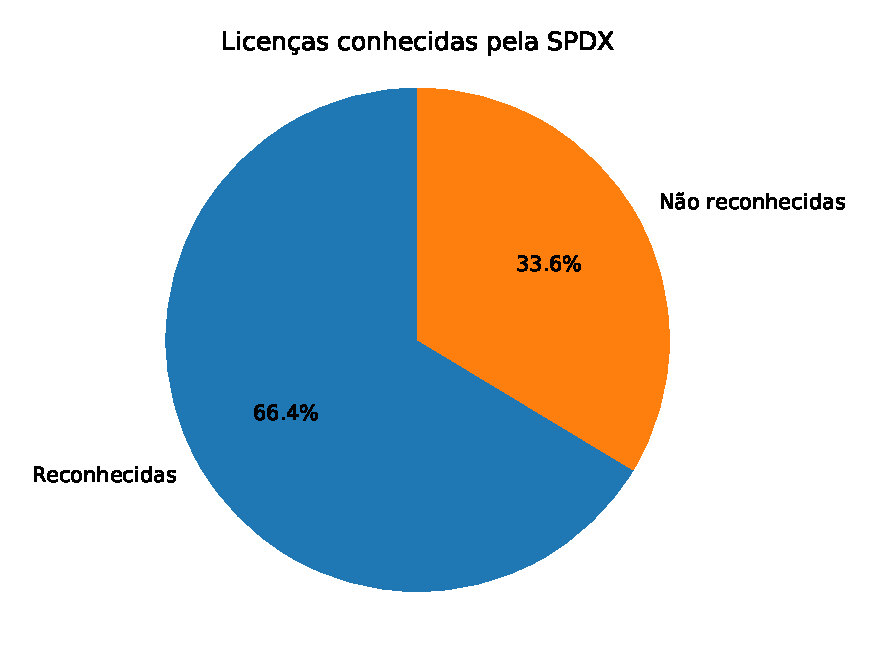
\includegraphics[scale=0.8]{figuras/resultados/pizza_licencas_conhecidas.eps}
	\fonte{Autoria própria.}
    \label{local-licencas-raiz}
\end{figure}

Como é possível observar, mais de 65\% (288 licenças) das licenças encontradas nos projeto são reconhecidas pela SPDX contra cerca de 35\% (146 licenças) não foram reconhecidas pela SPDX. \gnote{pq esses numeros nao abtem no numero total de licencas? descrever no texto} 

\gnote{descrever aqui as licenças não reconhecidas. quais sao? ao menos as tres mais utilizadas}

% COMPATIBILIDADE DE LICENÇAS ---------------------------------------------------
\subsection{Qual a quantitativo de licenças permissivas e restritivas?}\label{sec:comp}

Por fim, foi feita uma análise com o intuito de esclarecer o quantitativo de licenças permissivas e restritivas. Por licenças restritivas, entende-se \gnote{complementar}. Por licenças restritivas, entende-se \gnote{complementar}. Figure~\ref{local-licencas-raiz} apresenta os resultados.

\gnote{aqui tem que descrever melhor.. nao é o caso em que *no mesmo projeto* sao utilizados dois tipos de licenças diferentes? descreva como isso foi feito...}

\begin{figure}[H]
    \centering
    \caption{Compatibilidade de licenças encontradas no projeto}
    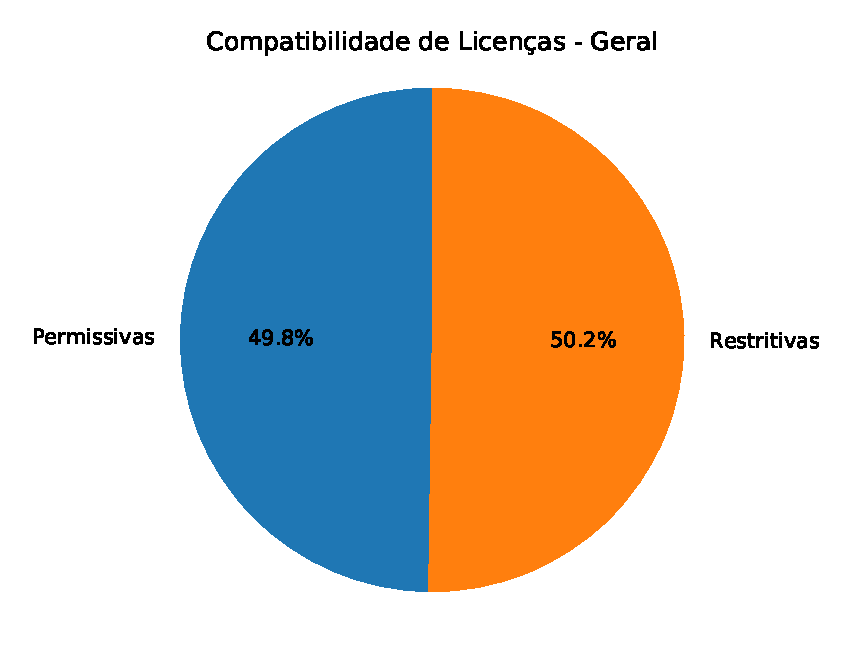
\includegraphics[scale=0.8]{figuras/resultados/pizza_compatibilidade_geral.eps}
	\fonte{Autoria própria.}
    \label{local-licencas-raiz}
\end{figure}

Rastreando todas as licenças encontradas no projeto de forma geral (licenças na raiz e em diretórios secundários), observou um empate em quantitativo de licenças que são compatíveis e não compatíveis nos projetos. Sendo que 50,5\% (780 licenças) permissivas e 49,5\% (765 licenças) são restritivas.

\begin{figure}[H]
    \centering
    \caption{Compatibilidade de licenças encontradas na raiz do projeto}
    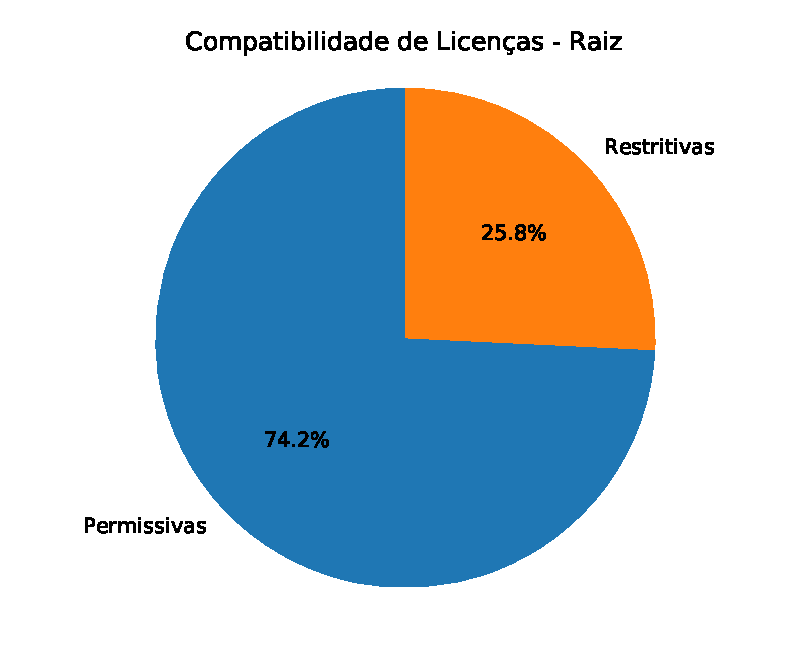
\includegraphics[scale=0.8]{figuras/resultados/pizza_compatibilidade_raiz.eps}
	\fonte{Autoria própria.}
    \label{local-licencas-raiz}
\end{figure}

Quando a busca foi restrita apenas as licenças encontradas na raiz dos projetos o panorama mudou, pois apenas 25\% das licenças encontradas eram incompatíveis. Sendo que 76,3\% (1.179 licenças) são compatíveis e 23,7\% (366 licenças) não são compativeis.

%comentario inicial=====================
\begin{comment}

% CATEGORIA DAS LICENÇAS ---------------------------------------------------
\section{Como as licenças encontradas podem ser categorizadas?}
Foi analisado os resultados da ferramenta com o intuito de esclarecer o tipo das licenças encontradas. Com essa analise podemos observar que a maioria das licenças são do tipo permissiva

\begin{table}[h]
	\centering
	\caption{Categoria das licenças encontradas.}
	\label{tab:categiorias}	
	    \begin{tabular}{l c c}
        \hline Categorias & Quantitativo Absoluto & Quantitativo Percentual (\%)\\
        \hline        
Permissive                & 193.899                & 74,80                          \\
Unstated License          & 19.202                 & 7,41                          \\
Copyleft Limited          & 14.290                 & 5,51                         \\
Patent License            & 10.634                 & 4,10                       \\
Copyleft                  & 10.257                 & 3,96                     \\
Source-available          & 7.194                  & 2,78                  \\
Public Domain             & 2.826                  & 1,09                  \\
Proprietary Free          & 809                    & 0,31                       \\
Free Restricted           & 52                     & 0,02                        \\
        \hline
Total                     & 259.214                & 100,00                      \\
        \hline
    \end{tabular}
	\fonte{Autoria própria.}
\end{table}


As licenças encontradas foram categorizadas conforme metodologia da ferramentas, essas categorias tem os seguintes significados:

\subsection {Permissive}
Software de código aberto disponibilizado sob licenças "não copyleft".
Isso geralmente exige a atribuição do código aberto incluído e pode incluir outras obrigações.

\subsection {Unstated License}
Software de terceiros com aviso de direitos autorais, mas sem licença declarada.
Exemplos comuns incluem trechos de código de publicações e sites (como os da O'Reilly Media).
A ausência de uma licença representa um risco de que o proprietário dos direitos autorais possa reivindicar obrigações de licença em algum momento futuro.
As equipes de produtos podem precisar entrar em contato com o proprietário dos direitos autorais para determinar as obrigações de licença, se houver.
Nessa categoria de licencas foram encontradas as seguintes licenças:

\subsection {Copyleft Limited}
Uma licença que exige que você redistribua o código-fonte, incluindo suas alterações, e também forneça atribuição aos autores do software.
Sua obrigação de redistribuir o código-fonte, incluindo o código proprietário vinculado ao código sob esta licença, é limitada de acordo com as regras específicas da licença.
Nessa categoria de licencas foram encontradas as seguintes licenças:

\subsection {Patent License}
Uma licença que se aplica a patentes em vez de software específico.
Pode ser usado em conjunto com outras licenças de software que se aplicam a um componente de software

\subsection {Copyleft}
Software de código aberto com uma licença "copyleft" que oferece permissão irrevogável ao público para copiar e redistribuir o trabalho da mesma forma ou modificado, mas com as condições em que todas essas redistribuições disponibilizam o trabalho em um formato que facilita modificações e uso adicionais os mesmos termos da licença.
Uma licença copyleft pode exigir que o código que interage com o código licenciado copyleft seja licenciado da mesma maneira.

\subsection {Source-available}
O software disponível na fonte é um software liberado por meio de um modelo de distribuição de código-fonte que inclui disposições em que a fonte pode ser visualizada e, em alguns casos, modificada, mas sem necessariamente atender aos critérios a serem chamados de fonte aberta.

\subsection {Public Domain}
Software de código aberto disponibilizado sem obrigações explícitas, mas com um aviso de licença que deve ser mantido com o código por política da organização.
A correspondência pode ser com software, exemplos de código em um site, especificações de domínio público publicadas ou outro tipo de publicação

\subsection {Proprietary Free}
Software gratuito proprietário que pode não exigir uma licença comercial, mas pode ter termos e condições específicos que as equipes de produto são obrigadas a seguir.
Alguns desses termos e condições são fornecidos com ou no código ou em licenças baixadas clicáveis.
Exemplos são o Contrato de Licença de Código Binário da Sun ou um BSP oferecido gratuitamente.

\subsection {Free Restricted}
Uma licença de estilo permissivo, que contém restrições sobre o uso do software (por exemplo, quando o software não se destina ao uso em usinas nucleares) ou o
redistribuição do software (por exemplo, onde a redistribuição comercial do software não é permitida sem permissão expressa).
A Free Software Foundation (FSF) diz que uma licença com esse tipo de restrição não é realmente de código aberto, embora o ponto de vista da OSI não seja tão rigoroso.

\end{comment}
%comentario final =====================